% !TeX program = xelatex
% !BIB program = biber

\documentclass[spanish]{textolivre}

% metadata
\journalname{Texto Livre}
\thevolume{18}
%\thenumber{1} % old template
\theyear{2025}
\receiveddate{\DTMdisplaydate{2024}{8}{1}{-1}}
\accepteddate{\DTMdisplaydate{2024}{10}{7}{-1}}
\publisheddate{\today}
\corrauthor{Javier Gil-Quintana}
\articledoi{10.1590/1983-3652.2024.53823}
%\articleid{NNNN} % if the article ID is not the last 5 numbers of its DOI, provide it using \articleid{} commmand 
% list of available sesscions in the journal: articles, dossier, reports, essays, reviews, interviews, editorial
\articlesessionname{articles}
\runningauthor{Gil-Quintana et al.}
%\editorname{Leonardo Araújo} % old template
\sectioneditorname{Daniervelin Pereira}
\layouteditorname{João Mesquita}

\title{Redes comunicativas universitarias sNOOC por la educación mediática de la tercera edad}
\othertitle{Redes de comunicação universitária sNOOC para educação midiática de idosos}
\othertitle{sNOOC communicative networks for media education of the elderly}

\author[1,2]{Javier Gil Quintana~\orcid{0000-0003-0326-2535}\thanks{Email: \href{mailto:jgilquintana@edu.uned.es}{jgilquintana@edu.uned.es}}}
\author[2]{Eduardo García Blázquez~\orcid{0000-0003-1229-3229}\thanks{Email: \href{mailto:ed.garcia@invi.uned.es}{ed.garcia@invi.uned.es}}}
\author[2]{José Javier Hueso Romero~\orcid{0000-0003-1375-2028}\thanks{Email: \href{mailto:jjavierhuesoromero@invi.uned.es}{jjavierhuesoromero@invi.uned.es}}}
\author[1]{Luis Miguel Romero Rodríguez~\orcid{0000-0003-3924-1517}\thanks{Email: \href{mailto:luis.romero@urjc.es}{luis.romero@urjc.es}}}
\affil[1]{Universidad Rey Juan Carlos, Facultad Ciencias de la Comunicación, Madrid, España.}
\affil[2]{Universidad Nacional de Educación a Distancia, Facultad de Educación, Madrid, España.}

\addbibresource{article.bib}

\begin{document}
\maketitle
\begin{polyabstract}
\begin{abstract}
Los Nano Open Online Massive (NOOC) representan una modalidad formativa de corta duración, análoga a los MOOC. Sin embargo, se caracterizan por una mayor especialización y brevedad, típicamente de 20 horas. El proyecto objeto de esta investigación aplicada, denominado socialNOOC (sNOOC), busca potenciar el empoderamiento del alumnado en su rol de e-teacher y evaluar el impacto de su labor en la educación mediática inclusiva de la población de la tercera edad en España. La iniciativa, coordinada por 79 estudiantes de posgrado de la UNED (España), se fundamenta en el proyecto formativo basado en pedagogías inclusivas en el que se integra recursos generados con Inteligencia Artificial y Metaverso. El análisis del proyecto ha incorporado enfoques cuantitativos, examinando las interacciones en la plataforma de educación a distancia (EAD) donde se desarrollaron los sNOOC, así como cualitativos, a través de la observación virtual de los 8 cursos masivos, las producciones de aprendizaje y la evaluación de un grupo interdisciplinario de 22 docentes en innovación educativa en España y Ecuador. Los resultados evidencian que la labor de los e-teacher e interacción de las redes comunicativas en los sNOOC han incrementado tanto el compromiso con el proyecto, como la satisfacción derivada de la experiencia colaborativa.

\keywords{Alfabetización informacional \sep Tercera edad \sep Educación a distancia. Metodología mixta}

\end{abstract}

\begin{portuguese}
\begin{abstract}
Nano Open Online Massive (NOOC) representa uma modalidade de treinamento de curta duração, análoga aos MOOCs. No entanto, caracterizam-se por maior especialização e brevidade, normalmente 20 horas. O projeto objeto desta investigação aplicada, denominado socialNOOC (sNOOC), procura potenciar a capacitação dos alunos no seu papel de e-professores e avaliar o impacto do seu trabalho na educação mediática inclusiva para a população idosa em Espanha. A iniciativa, coordenada por 79 alunos de pós-graduação da UNED (Espanha), baseia-se no projeto de formação baseado em pedagogias inclusivas em que se integram recursos gerados com Inteligência Artificial e Metaverso. A análise do projeto incorporou abordagens quantitativas, examinando as interações na plataforma de educação a distância (EAD) onde foram desenvolvidos os sNOOCs, e qualitativa, por meio da observação virtual dos 8 cursos massivos, das produções de aprendizagem e da avaliação de uma abordagem interdisciplinar. grupo de 22 professores em inovação educacional na Espanha e no Equador. Os resultados mostram que o trabalho dos e-professores e a interação das redes de comunicação no sNOOC aumentaram tanto o compromisso com o projeto como a satisfação derivada da experiência colaborativa.

\keywords{Alfabetização informacional\sep Terceira idade \sep Educação a Distância \sep Metodologia mista}

\end{abstract}
\end{portuguese}


\begin{english}
\begin{abstract}
Massive Nano Open Online Courses (MOOCs) are a short training modality similar to MOOCs, however they are characterized by greater specialization and brevity, usually lasting during the course of 20 hours. SocialNOOC (sNOOC) aims at empowering students to assume the role of e-teachers and assessing their contributions to the integrated media education of the elderly population in Spain through their work as e-teachers. This initiative is coordinated by 79 graduate students from the UNED (Spain) based on a training project integrating artificial intelligence and metaverse technology into pedagogical practices. Through the virtual observation of 8 massive courses, the learning productions, and the evaluation of an interdisciplinary group of 22 teaching experts in educational innovation in Spain and Ecuador, the project tters analyzed using quantitative approaches, examining interactions within the distance education platform (EAD), where the sNOOCs were developed, as well as qualitative approaches. The results show that the work of the e-teachers and the interaction of the communication networks in the sNOOCs have increased both the commitment to the project and the satisfaction derived from the collaborative experience.

\keywords{Information literacy \sep Third age \sep Distance education \sep Mixed methodology}
\end{abstract}
\end{english}
\end{polyabstract}

% !TeX root = main.tex

\section{Introducción}\label{sec-introducción}

La educación mediática es un proceso pedagógico y comunicativo que busca
que la ciudadanía desarrolle habilidades críticas que permitan analizar
el universo de medios que se proyectan en la sociedad postdigital
\cite{Escaño_2023}. Esta perspectiva convierte este ámbito de la
alfabetización en un trabajo por la inclusión de todos los sectores de
la sociedad, especialmente los más vulnerables que, por unos u otros
motivos, no pueden acceder a determinada información o son más
susceptibles a los peligros de esta. La educación mediática apuesta, por
tanto, por la inclusión, al buscar la promoción de la equidad, la
diversidad y la participación en el proceso educativo cite{guillen2024}. La integración de los principios que
fundamentan la inclusión en un planteamiento mediático es fundamental
para conseguir que la ciudadanía desarrolle las competencias digitales y
mediáticas imprescindibles para poder sobrevivir a la brecha de la
sociedad posdigital, potenciando su pensamiento crítico y, en
consecuencia, su actitud crítica \cite{palacios-rodríguez2025}. En este contexto hipermediatizado, la educación mediática
proporciona oportunidades de aprendizaje a través de \emph{mass media} y
\emph{social media} de manera equitativa y accesible, incluidas aquellas
personas que, debido a su edad, han sido excluidas o marginadas del
proceso de digitalización.

La Educación Abierta y a Distancia (EAD) ha jugado un papel importante
en el ámbito de la educación mediática y, como consecuencia, en la
creación de redes comunicativas globales al posibilitar la conexión de
estudiantes de distintas ubicaciones geográficas y contextos culturales.
La UNED desempeña un papel destacado desde 1972 en España promocionando
y desarrollando este modelo formativo y el acceso a la educación
superior de calidad a un amplio abanico de personas. Más
específicamente, en el ámbito de la EAD, la UNED ha colaborado
activamente por la incursión de la educación mediática, a través de los
\emph{Massive Open Online Courses} (MOOC), ofreciendo éstos a través de
su plataforma Uned Abierta, o de otras conocidas como \emph{Coursera},
\emph{edX}, \emph{Miriadax}, \emph{EcoDigitalLearning,} tmooc.es, etc.,
contribuyendo así al intercambio de conocimiento y la
internacionalización de la universidad. Este modelo formativo, diseñado
desde hace más de quince años (Ratnasari; Chou; Huang, 2024), puede
colaborar en la promoción de la inclusión social, al ofrecer un acceso
global, flexibilidad, costos reducidos, adaptabilidad, diversidad de
temáticas, interacción, participación y construcción colectiva del
conocimiento. Se promueve así un aprendizaje a lo largo de la vida
buscando la convergencia mediática: vídeos, lecturas, cuestionarios,
foros, recursos gamificados, creaciones con IA \cite{Aparicio-Gómez2024,cárdeasbenavides2024} e incluso
entornos inmersivos incluyendo los metaversos \cite{huesoromero2024,chuchuca2024metaverso}.

En el presente estudio hemos optado, dentro de las diferentes tipologías
de los MOOC, por el modelo sNOOC \cite{quintana2024snooc}. Tradicionalmente,
se han presentado los SPOC, xMOOC, cMOOC, sMOOC, tMOOC, COMOOC, pero,
actualmente también nos encontramos con los \emph{Nano Open Online
Courses} - NOOC \cite{clark2013moocs,gomez2016,Osuna-Acedo2017,LopezdelaSerna_Garrido_2018,Escaño_Dewhurst_2024}, un planteamiento
concreto y personalizado que estructura su duración en horas y articula
su estructura en torno a un contenido, herramienta o habilidad concreta
\cite{MANANGÓN-CABRERA2023,huesoromero2024}; con una duración máxima de veinte
horas \cite{intef2016}. Una formación en módulos comunicativos e
interactivos más minimalista que se presenta como novedosa, líquida y
flexible de contenidos, de recursos, de espacio y de tiempo \cite{basantes2020}. Perfilando aún más
nuestra elección, hemos apostado en el estudio por los sNOOC o
\emph{social}NOOC que posibilitan más aún el empoderamiento social de
redes comunicativas de estudiantes gracias a la creación colectiva del
conocimiento, la base de la cultura participativa y la apuesta por la
fidelización-compromiso del alumnado convertido en \emph{e-teacher}.
Esta implementación de los sNOOC se presenta como herramienta de
evaluación continua en la EAD, centrándose en experiencias y
valoraciones del alumnado, los elementos comunicativos y pedagógicos,
así como el proceso de construcción colaborativa de los contenidos,
poniendo énfasis en pedagogías inclusivas, que se enriquecen de las
metodologías activas, la creación con IA y metaverso \cite{galíndez2024}. Estas prácticas pedagógicas inclusivas, desde un diseño universal
de aprendizaje \cite{SanchezFuentes2023}, valoran la diversidad de
habilidades, intereses, experiencias y estilos de aprendizaje,
garantizan la equidad, aseguran la adaptabilidad utilizando estrategias
flexibles adaptadas a las diversas capacidades, promueven la
participación, fomentan la colaboración de la comunidad virtual y la
creación de entornos seguros, acogedores y estimulantes.

En este artículo presentamos el análisis de una experiencia que parte de
la creación de redes comunicativas en estudiantes de posgrado de la
Universidad Nacional de Educación a Distancia (UNED) con la finalidad de
convertirlos en \emph{e-teacher,} implementando proyectos formativos
para que las personas de la tercera edad, en riesgo de exclusión
digital, adquieran competencias mediáticas. La creación de esta red
comunicativa sólida parte de un espacio académico de la asignatura de
``Escenarios virtuales para la participación'' y se proyecta como
vinculación y transferencia a la sociedad. Los recursos comunicativos
cobran protagonismo en estas redes, no sólo a través de la plataforma
del curso concreto, sino también en la creación con el uso de la
Inteligencia Artificial (IA) o de espacios inmersivos de una plataforma
sNOOC, donde no sólo las personas participantes puedan formarse, sino
también puedan conectarse, discutir temas relevantes, compartir recursos
o difundir por el \emph{software} social ideas originales. Este proyecto
formativo lleva a la potencialización de la mentoría entre iguales,
unidos en red de intereses y en diversidad de propósitos, donde se
establecen relaciones más cercanas entre el alumnado y el aprendizaje
colaborativo.

La formación mediática de personas de un sector, que se puede considerar
a nivel mediático en peligro de exclusión, como es el de la tercera
edad, es un reto que ya han iniciado otros agentes educativos y sociales
desde diferentes instituciones \cite{abad-acala2014,abad-acala2017,Leal-Maridueña2017,heredia-sánchez2023}. En este caso
concreto, se ha visto beneficiada gracias a la solidaridad y
empoderamiento de redes de estudiantes unedianos \cite{Swan2015,Reich2015}, y el
compromiso por la formación mediática, promoviendo un mejor sentido de
la responsabilidad cívica \cite{bringle1996}, convirtiéndose en un
planteamiento pionero en esta etapa de formación. En esta experiencia,
el compromiso se materializa como un puente tangible que vincula la
formación a través de sNOOC con las problemáticas sociales como es la
alfabetización mediática de las personas de la tercera edad, pocas veces
productoras o creadoras de contenidos y muchas más consumidoras pasivas
de las redes sociales, en comparación con generaciones más jóvenes,
sobre todo en plataformas como Instagram, TikTok, YouTube, X o Facebook.
Los adultos mayores suelen comunicarse a través de estas interfaces con
amistades y familiares, comparten recuerdos, siguen noticias o temas
interesantes, e incluso, las y los más valientes, se animan a formar
parte de comunidades. Las plataformas, conocedoras de esta situación,
están adaptando sus interfaces y servicios para ser más accesibles y
fáciles de usar para personas de estas edades. Partiendo de esta
realidad inequitativa se puede y se debe impulsar, a través de proyectos
formativos de alfabetización mediática como el que presentamos en esta
investigación, una mejora de las habilidades, competencias y capacidades
de este grupo demográfico, especialmente afectado por la brecha digital
generacional.

% !TeX root = main.tex

\section{Metodología}\label{sec-metodología}

La metodología de la investigación la entendemos como el conjunto de
procedimientos y técnicas que el equipo investigador ha utilizado en el
diseño, desarrollo y análisis del estudio. En este caso concreto, el
método utilizado ha sido de corte mixto, utilizando técnicas
cualitativas y cuantitativas. Las cualitativas se han basado en la
etnografía virtual de los datos generados en los sNOOC y las
conclusiones del juicio del equipo de expertos. Las cuantitativas
provienen de los cuestionarios de satisfacción del alumnado y de los
datos de interacción del alumnado en la plataforma de aprendizaje.


\subsection{Objetivos e hipótesis}\label{sub-sec-objetivosehipotesis}

El objetivo general de este estudio es analizar el proceso de creación
de redes comunicativas de estudiantes para la implementación de sNOOC
como método de evaluación continua en la UAD y su repercusión en la capa
social como modelo de formación mediática en personas de la tercera
edad. Con base en este objetivo general, los objetivos específicos hacen
referencia a:

\begin{itemize}
\item
Objetivo Específico 1 (OE1): Investigar las percepciones y opiniones
de las redes comunicativas de estudiantes respecto a la utilidad y
efectividad de un sNOOC como método de evaluación continua y su
impacto en la motivación hacia el aprendizaje.
\item
Objetivo Específico 2 (OE2): Examinar el proceso de desarrollo de las
redes comunicativas de estudiantes para la creación de contenidos de
los sNOOC, centrándose en el impacto del uso de pedagogías inclusivas,
IA y Metaverso en EAD.
\item
Objetivo Específico 3 (OE3): Evaluar el nivel de implicación activa de
las redes comunicativas de estudiantes en la plataforma de la UNED y
en la creación colaborativa del sNOOC en tmooc.es.
\end{itemize}

A continuación, se formulan las hipótesis para dar respuesta a las
relaciones causales:

\begin{itemize}
\item
Hipótesis 1 (H1-OE1): Si las redes comunicativas de estudiantes
perciben el sNOOC como una herramienta efectiva y útil para la
evaluación continua, aumentará su motivación intrínseca hacia el
aprendizaje y su participación en las actividades y recursos del
itinerario de aprendizaje propuesto.
\item
Hipótesis 2 (H2-0E2): Si el modelo sNOOC es diseñado y aplicado
considerando criterios pedagógicos inclusivos y herramientas
tecnológicas adecuadas, mejorará la comprensión de los contenidos por
parte de las redes comunicativas de estudiantes, incrementando su
satisfacción general con la experiencia de EAD.
\item
Hipótesis 3 (H3-OE3): Si el itinerario de aprendizaje en sNOOC está
basado en pedagogías inclusivas, se incrementará el compromiso activo
de las personas participantes, reflejado en una mayor interacción,
colaboración en equipo y corresponsabilidad en la construcción
colectiva del conocimiento.
\end{itemize}


\subsection{Muestra, instrumentos y análisis de
	datos}\label{sub-sec-muestrainstrumentos}
	
	El objeto de estudio de esta investigación son las interacciones del
	alumnado en la plataforma ALF de la UNED, contando con la participación
	de 79 personas, 57 mujeres y 22 hombres; 1 de nacionalidad croata y, el
	resto, española. Estos participantes han sido estudiantes del Máster
	Universitario en Educación y Comunicación en la Red y, dentro de este,
	de la asignatura ``Escenarios Virtuales para la participación'', una
	disciplina con contenidos relacionados con la educación mediática. En
	este caso concreto, para estructurar el método cuantitativo, se han
	utilizado los cuestionarios con preguntas diseñadas para recopilar datos
	cuantitativos correspondiente al curso 2023/2024.
	
	Referido a la plataforma ``tmooc.es'' donde este grupo de estudiantes
	creó los sNOOC, se ha realizado un análisis de estas propuestas tomando
	también esos entornos como objeto de estudio. Se tuvieron en cuenta los
	registros de datos relacionados con la dedicación en la creación de los
	sNOOC. Los sNOOC seleccionados son los siguientes: ``Introdúcete al
	mundo de Facebook'' (sN1), ``Senior 3.0'' (sN2), ``Correo electrónico
	son misterios: alfabetización digital para personas mayores'' (sN3),
	``Enredados en la edad dorada: dominar Facebook e Instagram con
	confianza'' (sN4), ``Healthy seniors network'' (sN5), ``Estas a un clic
	de conocer el mundo digital'' (sN6), ``Familias y aprendizaje en red''
	(sN7) y ``Google e inteligencia artificial, tus compañeros digitales''
	(sN8). En cuanto al enfoque cualitativo, se consideraron los datos
	generados a través de los sNOOC y las conclusiones del juicio de 22
	personas expertas internacionales, con el fin de validar hipótesis y
	evaluar riesgos o problemáticas presentes en el proyecto formativo. Para
	analizar los datos cuantitativos y cualitativos se utilizaron los
	programas SPSS y Atlas.ti, respectivamente. Estos aspectos se han
	organizado en categorías que se ajustan a las dimensiones de la
	educación inclusiva.

% !TeX root = main.tex


\section{Resultados}\label{sec-resultados}
Los resultados de este estudio se han organizado en torno a dos
categorías fundamentales. En primer lugar, la Categoría 1 hace
referencia a ``Acceso, equidad y participación''; y, en segundo lugar,
la Categoría 2, se refiere a ``Respecto a la diversidad, colaboración y
prácticas pedagógicas inclusivas''. Estas dimensiones son
interdependientes y mantienen sinergias con el fin de promover la
equidad, la diversidad, la participación y el éxito del proyecto de
alfabetización mediática para personas de la tercera edad.
	

\subsection{Categoría 1: Acceso, equidad y participación}\label{sub-sec-categoría}
	

\subsubsection{Subcategoría: Acceso a la plataforma digital}\label{sub-sub-sec-subcategoríaacessoala}
	
El acceso a la plataforma de la asignatura ``Escenarios Virtuales para
la Participación'' desde donde se ha proyectado la red comunicativa nos
da a conocer, a nivel de tiempo y dedicación, la actuación como
interactuados de las y los estudiantes, tanto en términos de frecuencia
como de tiempo dedicado. El análisis de los datos de acceso y
participación revela diversos patrones: determinados estudiantes
muestran registros de acceso mínimos, en contraste, otras y otros
estudiantes con niveles de acceso significativamente altos, con datos
que acceden a 3436 y 1981 respectivamente. La cantidad de sesiones varía
también significativamente, con estudiantes que participan en 736 y 123
sesiones respectivamente, lo cual, indica un rol de interactuado
frecuente y prolongado en la plataforma. En este sentido, el acceso nos
remite a la posible participación, otro aspecto de esta categoría,
reflejando diversidad de hábitos de estudio y nivel de compromiso del
alumnado.
	
Los datos recopilados se han analizado en tres métricas que hacen
referencia a accesos, minutos y sesiones. El valor medio sugiere que, en
promedio, se han efectuado 520 accesos, utilizando 2575 minutos y
desarrollándose unas 41680 sesiones. La mediana, representando el valor
central de los datos ordenados, muestra que la mitad de los valores se
sitúan encima y la otra mitad por debajo de 3755 accesos, 20 minutos y
25 sesiones. El valor modal, es decir, aquel que aparece con mayor
frecuencia, señala que el número más común de accesos es 2, mientras que
los valores predominantes para el tiempo y el número son 0 minutos y 1
sesión. El total acumulado de accesos, minutos y sesiones es 43695, 2163
y 3501. Los valores mínimos y máximos ilustran el rango de los datos,
con un mínimo de 1 acceso y un máximo de 3436.
	
En términos de tiempo, el mínimo registrado es 0 minutos, indicando
periodos de inactividad, mientras que el máximo es 96 minutos.
Concretamente, para el tiempo dedicado a las sesiones, el rango es
variable, entre 1 y 736. Estos datos, representados en la \Cref{fig-01},
ofrecen una comprensión detallada de la actividad de acceso, el tiempo
dedicado y el número de sesiones, esencial para analizar las
interacciones y los patrones de comportamiento del alumnado en la
plataforma. Con base en los datos sobre el tiempo de permanencia en la
plataforma, según la \Cref{fig-02}, se observa una distribución heterogénea
en las horas dedicadas al estudio por parte de las personas que forman
la red comunicativa. Un 38,9~\% dedica entre 2 y 4 horas de estudio; un
27,8~\% entre 2 y 4 horas; un 16,7\% de las personas participantes entre
6 y 8 horas; y un 11,1~\% reporta estudiar más de 8 horas.
	
\begin{figure}[htbp]
\centering
\begin{minipage}{.85\textwidth}
\caption{Tiempo accesos minutos.}
\label{fig-01}
\includegraphics[width=\textwidth]{Imagem1.png}
\source{Elaboración propia.}
\end{minipage}
\end{figure}
	
\begin{figure}[htbp]
\centering
\begin{minipage}{.85\textwidth}
\caption{Tiempo de estudio.}
\label{fig-02}
\includegraphics[width=\textwidth]{Imagem2.png}
\source{Elaboración propia.}
\end{minipage}
\end{figure}		

Al referirnos a la valoración global de la asignatura, nos proporciona
una información valiosa sobre aspectos de la equidad en el contexto
educativo. Según se presenta en la \Cref{fig-03} sobre los tramos de ítem,
los resultados muestran una progresión, destacando una mayor atención a
la adecuación, coherencia y satisfacción global. El tramo 1, la mediana
es 14,4, con un rango intercuartílico (IQR) desde 5,6 hasta 44,4; en el
tramo 2, la mediana es de 15,7, con un IQR desde 5,6 hasta 43,9; en el
tramo 3, la mediana es de 41,0, y el IQR abarca desde 27,8 hasta 55,6;
en el tramo 4, la mediana se encuentra en 33,3, con un IQR desde
aproximadamente 5,6 hasta 55,6. En los tramos 1, 2 y 4 se identifican
valores atípicos en ambos extremos.
	
\begin{figure}[htbp]
	\centering
    \begin{minipage}{.85\textwidth}
	\caption{Valoración de la asignatura.}
	\label{fig-03}
	\includegraphics[width=\textwidth]{Imagem3.png}
	\source{Elaboración propia.}	
    \end{minipage}
\end{figure}
	
\subsubsection{Subcategoría: Equidad en el acceso, desempeño y evaluación}\label{sub-sub-sec-equidadenelacceso}
	
Según se evidencia en la \Cref{fig-04}, tramo 1, el alumnado muestra un mayor
nivel de conocimientos previos (44,4~\%), con adecuación entre la carga
de trabajo y créditos de la asignatura (16,7~\%). En el tramo 2 la
satisfacción global sobre los recursos y apoyo (50~\%) y utilidad del
plan de trabajo para la preparación de la asignatura (27,8~\%) son
aspectos bien valorados. En el tramo 3, resalta la coherencia de los
contenidos con el conjunto del máster (38,9~\%); y la percepción
equitativa sobre los datos contenidos en la guía de estudio (44,4~\%).
En el tramo 4, la satisfacción global con el equipo docente (55,6~\%) y
la atención inclusiva que el mismo presta a los foros (47,1\%) son
aspectos altamente valorados. Se observa una distribución variada en la
valoración de la asignatura en diferentes aspectos y tramos, lo que
sugiere que la percepción de las y los estudiantes puede verse
influenciada por diferentes factores a lo largo del curso.
	
\begin{figure}[htbp]
\centering
\begin{minipage}{.85\textwidth}
\caption{Valoración de asignatura por tramos.}
\label{fig-04}
\includegraphics[width=\textwidth]{Imagem4.png}
\source{Elaboración propia.}	
\end{minipage}
\end{figure}
	
En lo atinente a la valoración de la asignatura en relación con otras,
se puede verificar según presenta la \Cref{fig-05} que esta disciplina recibe
valoraciones bastante altas en todos los ítems evaluados, con puntajes
que oscilan entre 36,15~\% y 81,7~\%, observando una percepción positiva
en cuanto a la interacción que se proyecta. Aspectos como "La coherencia
de los contenidos de la asignatura con el conjunto del máster" y "Los
conocimientos adquiridos en esta asignatura", son más altas, indicando
una fuerte percepción de coherencia y utilidad de los contenidos en
relación con el programa y un alto grado de aprendizaje. Otras
referencias a "La adecuación del material didáctico para el estudio de
esta asignatura" y "La utilidad del curso virtual para la preparación de
la asignatura" muestran puntajes más bajos, indicando que podría haber
margen de mejora sobre la calidad y la utilidad de las herramientas
comunicativas y recursos presentados. Los ítems tienen un margen de
error estimado medio o bajo, lo que sugiere que las estimaciones de las
puntuaciones son bastante precisas y fiables. Esta disciplina está bien
valorada y aumenta su valoración cada año, según presenta la \Cref{fig-06},
con ámbitos específicos que podrían beneficiarse a nivel de inclusión
como las herramientas comunicativas, los recursos y la metodología.
	
\begin{figure}[htbp]
	\centering
    \begin{minipage}{.85\textwidth}
	\caption{Valoración de asignatura en relación con otras.}
	\label{fig-05}
	\includegraphics[width=\textwidth]{Imagem5.png}
    \source{Elaboración propia.}
    \end{minipage}
\end{figure}

\begin{figure}[htbp]
	\centering
    \begin{minipage}{.85\textwidth}
	\caption{Valoración de asignatura por año.}
	\label{fig-06}
	\includegraphics[width=\textwidth]{Imagem6.png}
	\source{Elaboración propia.}
    \end{minipage}
\end{figure}
	
En la \Cref{fig-07} se pone de manifiesto cómo el alumnado distribuye su
tiempo, lo que puede reflejar la accesibilidad a los recursos y el
tiempo de desempeño. Los documentos, las tareas y calificaciones son las
herramientas que requieren más tiempo, con 4190 y 2202 minutos
respectivamente.

\begin{figure}[htbp]
\centering
\begin{minipage}{.85\textwidth}
\caption{Tiempo accesos minutos por recurso.}
\label{fig-07}
\includegraphics[width=\textwidth]{Imagem7.png}
\source{Elaboración propia.}
\end{minipage}
\end{figure}
	

\subsubsection{Subcategoría: Participación y red comunicativa}\label{sub-sub-sectionparticipación}
	
El análisis de los diferentes textos que se presentan en los foros de la
plataforma nos otorga información clave sobre el proceso de creación de
la red que se puede estructurar en torno a cinco puntos:
	
\begin{itemize}
\item
Búsqueda y formación de grupos: personas participantes están buscando
semejantes con intereses similares.
\item
Presentación personal: cada persona ofrece una breve presentación,
destacando su experiencia, formación y motivaciones para unirse al
proyecto de formación mediática. Esto ayuda a crear una red específica
teniendo presente los antecedentes y perspectivas personales.
\item
Diversidad de participantes: las personas provienen de lugares
geográficos distintos, con diferentes áreas de especialización como
enseñanza de idiomas, tecnología educativa, pedagogía, etc. Así, las
discusiones son más enriquecedoras y los proyectos formativos con
variedad de perspectivas.
\item
Intereses comunes: a pesar de la diversidad formativa y de
proveniencia geográfica, tienen como interés común la pedagogía
digital, la tecnología educativa y la innovación en la enseñanza. Esto
consolida la red comunicativa en base a un objetivo concomitante.
\item
Inclusión, colaboración y apoyo mutuo: disposición a colaborar y
apoyarse mutuamente en la formación de grupos, reflejando espíritu
colaborativo y solidario intencional de cara al proyecto formativo que
se quiere desarrollar.
\end{itemize}

A juzgar por estas cuestiones analizadas, se puede comprobar cómo la
conversación desarrollada en el foro manifiesta un ambiente colaborativo
y participativo con un alumnado comprometido con la creación colectiva
del conocimiento y la aplicación práctica de los conceptos aprendidos en
el itinerario de aprendizaje. El uso intensivo de los foros es un
componente esencial en la organización de las redes comunicativas, base
del proyecto de alfabetización mediática.

Con una correlación positiva significativa entre accesos y sesiones ($r =
0.81$, $p < 0.001$), y una correlación moderada entre accesos y
minutos ($r = 0.5$, $p < 0.001$), nos indica que las personas
participantes, además de acceder a los foros con frecuencia, invierten
un tiempo considerable en ellos. Esto favorece la formación de grupos
con intereses similares y permite a cada participante destacar su
experiencia y motivaciones. A pesar de la diversidad de las y los
componentes de las diferentes redes, que provienen de diferentes lugares
y áreas de especialización, los intereses comunes fortalecen la red. La
disposición a colaborar y apoyarse mutuamente se refleja en el uso
intensivo de los foros, fomentando un espíritu de inclusión y
solidaridad en el proyecto formativo. La correlación moderada entre
minutos y sesiones ($r = 0.36$, $p = 0.001$) sugiere que un mayor tiempo en
los foros está asociado con un mayor número de sesiones. Sin embargo, el
número no muestra una relación significativa con accesos ($r = -0.04$, $p =
0.716$), minutos ($r = 0.07$, $p = 0.533$) o sesiones ($r = -0.09$, $p = 0.425$),
lo que indica que el número total de usuarios no afecta
significativamente estos parámetros. Esto subraya la importancia de la
calidad de la interacción sobre la cantidad de personas en el éxito del
proyecto formativo. La alta frecuencia de uso de los foros facilita
también la búsqueda y formación de grupos, donde las personas
participantes buscan intereses similares; refleja un espíritu de
inclusión, colaboración y apoyo mutuo, crucial para la formación de
grupos colaborativos y solidarios en el proyecto formativo, según
observamos en la \Cref{fig-08}.

\begin{figure}[htbp]
\centering
\begin{minipage}{\textwidth}
\caption{Interacción en los foros.}
\label{fig-08}
\includegraphics[width=\textwidth]{Imagem8.png}
\source{Elaboración propia.}
\end{minipage}
\end{figure}

El diagrama de Sankey, presentado en la \Cref{fig-09}, muestra cómo las y los
participantes, a través de su autoconocimiento y desarrollo personal,
buscan a semejantes con intereses similares para formar redes. Esto se
refleja en las conexiones que fluyen desde "Autoconocimiento" y
"Desarrollo personal" hacia otros nodos en el diagrama. En cuanto a la
``Presentación personal'', las y los participantes presentan sus
antecedentes y motivaciones, lo que ayuda a formar una red específica.
Esto se puede ver en las conexiones que fluyen desde "Autoconocimiento"
y "Desarrollo personal" hacia "Interacción" y "Motivación". En lo que
respecta a ``Diversidad de participantes'', aparece reflejada en el nodo
"Diversidad", enriquece las discusiones y los proyectos formativos. Las
conexiones que fluyen desde "Diversidad" hacia otros nodos indican cómo
ésta se integra en el proyecto. Con respecto a ``Intereses comunes'', a
pesar de la diversidad, las y los participantes tienen un interés común
en la pedagogía digital, la tecnología educativa y la innovación. Esto
se refleja en las conexiones que fluyen hacia y desde el nodo
"Educación". En cuanto a inclusión, colaboración y apoyo mutuo: la
disposición se refleja en el uso intensivo de los foros, promoviendo un
espíritu de inclusión y solidaridad en el proyecto formativo. Esto se
puede ver en las conexiones que fluyen hacia y desde el nodo
"Interacción".

\begin{figure}[htbp]
	\centering
    \begin{minipage}{\textwidth}
	\caption{Formación de redes comunicativas y conexiones de participantes.}
	\label{fig-09}
	\includegraphics[width=\textwidth]{Imagem9.png}
	\source{Elaboración propia.}	
    \end{minipage}
\end{figure}


\subsection{Categoría 2: Diversidad, colaboración y prácticas pedagógicas inclusivas}\label{sub-section-diversidad}
	
	
\subsubsection{Subcategoría: Plataforma digital para la diversidad}\label{sub-sub-sec-subcategoríaplataformadigital}
	
La plataforma ``tmooc.es'' donde se ha desarrollado este proyecto es
Chamilo, de código abierto y con múltiples funcionalidades para la
creación de sNOOC. Partiendo de un aspecto clave como es la diversidad,
analizamos si es real en el proyecto formativo y si se está garantizando
que todas las personas, independientemente de sus características o
capacidades, puedan ejercer el derecho a la inclusión y la igualdad de
oportunidades. Referido a la accesibilidad, Chamilo proporciona diversas
herramientas para la creación de contenidos accesibles desde el diseño
universal, incluyendo todo tipo de dificultad: contenido multimedia con
subtítulos, crear contenido estructurado y navegable, personalizar
diseño compatible con lectores de pantalla y otros asistentes
tecnológicos. Además, esta plataforma posibilita también el uso adecuado
de etiquetas semánticas HTML y descriptores de elementos multimedia.
	
Referido a los recursos generados, se ha utilizado la plataforma
Genially, considerándose un espacio accesible que garantiza su
usabilidad por personas con diversas capacidades, incluyendo en sus
recursos: compatibilidad con lectores de pantalla, controles de teclado,
contraste y tamaño del texto y compatibilidad con estándares web,
siguiendo las pautas de la W3C (\emph{World Wide Web Consortium}).
	
La aportación del juicio de expertos también ha tenido como finalidad
reconocer y valorar el entorno sNOOC como espacio de aprendizaje
accesible, equitativo y enriquecedor. Los principios clave de la
pedagogía inclusiva que se han tenido presentes han sido: la valoración
de la diversidad, la equidad, la adaptabilidad, la colaboración, la
participación activa y los ambientes de apoyo.
	

\subsubsection{Subcategoría: Colaboración y trabajo en equipo}\label{sub-sub-sec-subcategoríacolaboración}
	
La creación en los sNOOC presenta algunas correlaciones significativas,
especialmente entre el uso de lecciones y enlaces, entre el tiempo en el
curso y el uso de documentos. Así, se identifican correlaciones,
presentadas en la \Cref{fig-10}, entre diferentes variables relacionadas con
la participación en sNOOC y los valores \emph{p} asociados. Se destacan
correlaciones positivas significativas entre ``Lecciones y Enlaces'' ($r
= 0.73$, $p = 0.038$), lo que indica que a medida que los estudiantes
completan más lecciones, también tienden a utilizar más enlaces. Existe
una correlación positiva alta ($r = 0.66$, $p = 0.076$) entre ``Documentos''
y ``Tiempo en el curso'', y mínimamente significativa entre el uso de
documentos y el tiempo total en el curso, indicando que los estudiantes
que pasan más tiempo en el curso también tienden a interactuar más con
los documentos. Finalmente, existe una correlación muy alta ($r = 0.96$, $p
< 0.001$), entre el ``Tiempo'' en el curso y ``Tiempo'' medio
indicando que aquellos que pasan más tiempo total en el curso también
tienen un tiempo medio de sesión mayor. Por otro lado, no se identifican
correlaciones significativas entre las variables que tienen valores p
altos (mayores a 0.05), es decir, aquellas que no son estadísticamente
significativas. Por ejemplo, la correlación entre ``estudiantes'' y el
``tiempo en el curso'' ($r = 0.34$, $p = 0.412$) y las correlaciones entre
``lecciones'' y ``ejercicios'' ($r = 0.28$, $p = 0.505$), y entre ``foros''
y ``tareas'' ($r = 0.5$, $p = 0.204$) tampoco son estadísticamente
significativas. En cuanto a correlaciones negativas, se identifican
entre ``lecciones'' y ``tiempo'' en el curso ($r = -0.46$, $p = 0.252$) y
entre enlaces y tiempo en el curso ($r = -0.22$, $p = 0.594$) y entre el
``tiempo'' en el curso y los ``ejercicios'' ($r = -0.23$, $p = 0.576$) y
entre el ``tiempo'' en el curso y el ``glosario'' ($r = -0.26$, $p =
0.528$). Estas indican una relación inversa, aunque no son
estadísticamente significativas. Las actividades que implican
interacciones directas y frecuentes, como el uso de enlaces y
documentos, tienden a mostrar relaciones positivas con el tiempo total y
el tiempo medio en el curso. El alumnado que pasa más tiempo en el curso
suele interactuar más con estos recursos, aunque no todas estas
correlaciones son estadísticamente significativas.
	
\begin{figure}[htbp]
\centering
\begin{minipage}{\textwidth}
\caption{Participación en sNOOC.}
\label{fig-10}
\includegraphics[width=\textwidth]{Imagem10.png}
\source{Elaboración propia.}
\end{minipage}
\end{figure}
	
	
La mayoría de los sNOOC, según observamos en la \Cref{fig-11}, no utilizan
recursos evaluables, con excepción de ``sN2'' (18) y ``sN3'' (1), a
diferencia de ``sN6'' que tiene una cantidad muy alta de recursos
evaluables (93). En cuanto al empleo de los foros, está presente en
todos los cursos, siendo ``Estas a un click de conocer el mundo digital"
el que tiene mayor número (11); y menor cantidad ``sN5'' y ``sN2''. Respecto
a las tareas, la mayoría de los cursos tienen tareas, aunque ``sN1'' y
``sN3'' no, mientras que ``sN8'' tiene la mayor cantidad (16). Con respecto
al empleo de ``Documentos'', todos utilizan documentos, siendo ``sN7'' el
que tiene la mayor cantidad de documentos (18), ``sN5'' y ``sN4'' utilizan
el menor número (4 cada uno). En cuanto a ``Lecciones'', el curso que
tiene mayor número de lecciones es ``sN3'' con (28), y los que tienen
menor cantidad son: ``sN2'', ``sN7'', y ``sN8'' con 4.
	
El sNOOC ``sN7'' tiene el mayor número de estudiantes (26), y con menor
número ``sN5'' y ``sN8'' (9 y 7 respectivamente). El uso del Glosario tiene
una cantidad muy alta de entradas (63) en ``sN3'', los de menor número son
``sN2'', ``sN5'', y ``sN8'. En lo relativo al empleo de ejercicios, ``sN4''
tiene la mayor cantidad (22), ``sN8" no tiene. En cuanto al empleo más
alto de recursos, foros, tareas, documentos, lecciones y estudiantes, se
puede destacar ``sN6'' con alto número de recursos evaluables (93) y foros
(11); ``sN3'' muestra una alta interacción con 28 lecciones, 30 enlaces y
63 glosarios; ``sN8' tiene un elevado número de tareas (16) y un tiempo
medio significativo (0:17:30); ``sN7'' sobresale en la cantidad de
documentos (18). Esta información proporciona una visión clara de cómo
se estructuran y utilizan los recursos en cada sNOOC, reflejando las
diferencias en su diseño y enfoque pedagógico.
	
\begin{figure}[htbp]
\centering
\begin{minipage}{.85\textwidth}
\caption{Tiempo accesos minutos.}
\label{fig-11}
\includegraphics[width=\textwidth]{Imagem11.png}
\source{Empleo de recursos, foros, tareas, documentos, lecciones y estudiantes en sNOOC. }
\end{minipage}
\end{figure}
		
A través del diagrama de caja representado en la \Cref{fig-12}, y sobre lo
comentado anteriormente, se puede evidenciar que la mayoría de los
cursos están liderados por una red comunicativa entre 3 y 6 docentes,
con un valor medio de 4.38 y una desviación típica de 1.06, lo que
indica una cantidad bastante uniforme de docentes por curso. El uso del
calendario varía ampliamente entre los cursos, con algunos que no lo
utilizan y otros que lo hacen hasta 3 veces, reflejado en un valor medio
de 0.75 y una alta desviación típica. La frecuencia de anuncios también
varía considerablemente, con un valor medio de 1 y una desviación típica
que sugiere diferencias en la comunicación entre los cursos. Además,
existe una gran variabilidad en la cantidad de ejercicios asignados,
desde cursos sin ejercicios hasta aquellos con 26, lo que podría indicar
diferentes enfoques pedagógicos. En cuanto, a la cantidad de recursos
evaluables varía significativamente entre los cursos, lo que puede
reflejar distintos métodos de evaluación, cosa que ocurre de manera
similar a los recursos evaluables, las tareas presentan una amplia gama
en su número, lo que indica variaciones en la carga de trabajo asignada
a los estudiantes. El uso de foros es más consistente entre los cursos,
lo que indica que son una herramienta común de interacción. Por otro
lado, la cantidad de documentos utilizados muestra una alta
variabilidad, lo que podría reflejar la riqueza de material
proporcionado en cada curso. Por lo que respecta a la variabilidad en el
número de lecciones, indica diferentes volúmenes de contenido. Asimismo,
la cantidad de estudiantes por curso varía, pero se mantiene en un rango
que sugiere un tamaño de clase manejable. La utilización de enlaces
varía ampliamente, lo que puede indicar diferentes niveles de
interactividad en los cursos. En resumen, el diagrama de caja muestra
que hay una gran variabilidad en la estructura y utilización de recursos
en los cursos, reflejando diferencias en diseño y enfoque pedagógico.
	
\begin{figure}[htbp]
\centering
\begin{minipage}{.85\textwidth}
\caption{Variabilidad en la estructura y utilización de recursos en sNOOC.}
\label{fig-12}
\includegraphics[width=\textwidth]{Imagem12.png}
\source{Elaboración propia.}
\end{minipage}
\end{figure}
	
Para finalizar esta subcategoría debemos indicar que el sNOOC ``sN7",
``sN4'' e ``sN1'' han utilizado la red social de YouTube, Facebook y ha
creado metaverso, los dos primeros, además, Instagram; ``sN5'' aún no
tienen espacios; "sN8'' y ``sN6'' solo YouTube; ``sN3'' YouTube y
metaverso; ``sN2'' YouTube, WhatsApp y metaverso.
	

\subsubsection{Subcategoría: Prácticas pedagógicas inclusivas}\label{sub-sub-sec-subcategoría}
	
El gráfico de co-ocurrencias, muestra visualmente la interacción entre
los elementos de las pedagogías inclusivas y varios aspectos del proceso
de aprendizaje, incluyendo el juicio de expertos. Se destaca la
interdependencia entre las pedagogías inclusivas y los diversos
componentes del aprendizaje, en donde cada aspecto, ya sea la valoración
de la diversidad, la equidad, la adaptabilidad, la colaboración, la
participación activa o los ambientes de apoyo, se refuerza y complementa
mutuamente. Esto contribuye a crear una experiencia educativa integral y
accesible, según representa la \Cref{fig-13}. Cada uno de estos elementos
desempeña un papel esencial en la promoción de una educación inclusiva
efectiva. Entre los hallazgos se destaca la ``valoración de la
diversidad'' con fuertes conexiones con ``narrativa gamificada'' y
``satisfacción'', lo que indica que la apreciación de la diversidad
contribuye significativamente a la motivación y al disfrute del
aprendizaje; ``la equidad'' vinculada con la ``evaluación'' y
``ambientes de aprendizaje'', una evaluación justa y entornos de
aprendizaje equitativos son esenciales para la inclusión;
``adaptabilidad'' muestra una relación con la ``metodología'', lo que
implica la importancia de métodos flexibles que se adapten a las
necesidades del alumnado; la colaboración está conectada con la
``participación activa'', destacando trabajo en equipo, cooperación y
participación más significativa del alumnado; la participación activa se
asocia con la ``satisfacción'', resaltando que, cuando el alumnado se
involucra activamente en su aprendizaje, tiende a estar más satisfecho
con su experiencia educativa; los ambientes de apoyo tienen vínculos con
todos los elementos mencionados, subrayando que un entorno de apoyo es
fundamental para facilitar la inclusión y el éxito de todas las
prácticas pedagógicas.
	
\begin{figure}[htbp]
\centering
\begin{minipage}{\textwidth}
\caption{Juicio de expertos referido a pedagogías inclusivas y componentes de aprendizaje.}
\label{fig-13}
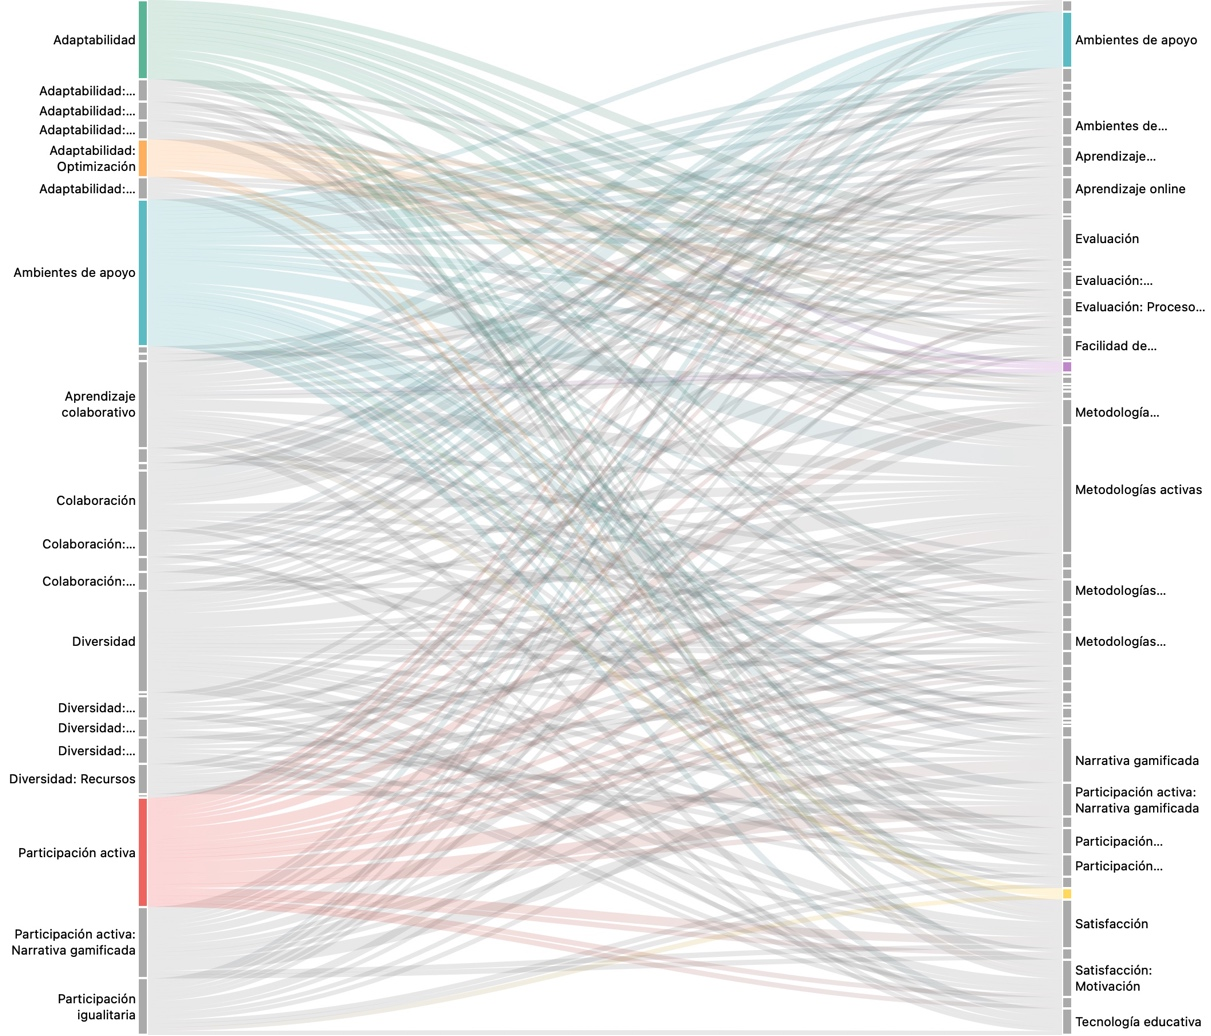
\includegraphics[width=\textwidth]{Imagem13.png}
\source{Elaboración propia.}
\end{minipage}
\end{figure}

\section{Discusión}\label{sec-discusión}

Las personas entrevistadas en ambas comunas de Chile han integrado las
tecnologías digitales a sus experiencias cotidianas. Sin embargo, esas
experiencias son afectadas por las brechas digitales estructurales
existentes, lo que genera como consecuencia, limitaciones para usar
tecnologías en contextos laborales \cite[P.11]{MORALES2020}.

La tendencia a no hacer usos complejos de tecnología y concentrarse en
experiencias de entretenimiento, se conecta con investigaciones previas
respecto a los ambientes digitales como mecanismos de evasión de la
realidad y con posibles efectos negativos, que orientan hacia un uso
excesivo y unívoco de redes sociales, con posibles efectos sobre la
salud mental de los usuarios \cite{CHARITSIS2022,XU2023}. Al mismo tiempo, estas prácticas, aunque actúan como una
limitación, tienen un potencial de convertirse en herramientas para
avanzar hacia procesos de alfabetización digital más complejos, en
particular las que se vinculan con búsqueda de información o
comunicación comunitaria.

En relación con las brechas digitales y sus causas estructurales, y del
mismo modo que los trabajos previamente citados de \textcite{PETHIG2021}
o \textcite{LONGORIA2022}, puede decirse que su manifestación es
multidimensional. El contexto territorial, la desigualdad económica,
educativa y de género, entre otros factores, generan efectos
acumulativos en el mundo digital. A lo anterior se suma la propia
situación de discapacidad debido a las brechas de diseño de
dispositivos, aplicaciones y sitios web \cite{EGARD2021,KELLY2016}.

Otra cuestión preocupante es la experiencia de temor a la tecnología que
algunas entrevistadas manifestaron. A diferencia de lo señalado por
\textcite{PETHIG2021}, que asocian la tecnología a la protección frente
al miedo de exponerse a la sociedad, en las entrevistas se manifiesta un
temor a los dispositivos y a su manipulación.

En este contexto, las entrevistas en ambas comunas dan cuenta de pocas
oportunidades formales de alfabetización digital, por lo que las
experiencias de uso de tecnologías en el trabajo son limitadas,
concentrándose en aquellos que tuvieron acceso a educación
técnico-profesional. De esta forma, se manifiesta una amplia disparidad
entre las competencias laborales demandas por el mercado laboral y las
posibilidades de alfabetización disponibles en sus contextos locales. El
contexto de brechas digitales estructurales y las limitaciones de acceso
a alfabetización digital, son coincidentes con lo señalado por \textcite{QU2022}
respecto a la precarización laboral, baja calificación y remuneración.

Debido al diseño de sitios web gubernamentales que no cumplen los
criterios establecidos en las propias normativas, y de forma similar a
lo señalado por \textcite{LIN2018}, puede decirse que hay políticas de
accesibilidad, pero baja implementación. En contraste con ese déficit en
la política nacional, la accesibilidad proviene de políticas comunales
que facilitan la conectividad, y que a su vez tienen un potencial de
vinculación comunitaria, en la que las PeSD pueden acceder a internet,
espacios de encuentro comunitario y con potencial para la formación de
competencias digitales para el trabajo.

Lo anterior implica el desafío de diseñar estrategias de política para
enfrentar la inevitable penetración de las tecnologías digitales en
todos los ámbitos de la vida, y especialmente en el mundo del trabajo
\cite{PEREZROLDAN2021}.

De acuerdo con \textcite[p. 4438]{LIN2018}, la inclusión no es
exclusivamente un esfuerzo de política pública, sino más bien de
transformación de la sociedad. En ese mismo sentido apunta el trabajo de
\textcite[p. 3]{KOLOTOUCHKINA2022} que identifican cuatro
áreas para la inclusión digital: políticas de equidad digital, políticas
de estandarización, construcción de una cultura de accesibilidad
universal y compromisos sociales compartidos por el Estado, el sector
privado y la sociedad civil.

Finalmente, es importante considerar las limitaciones de la
investigación. Como se ha señalado, la investigación previa sobre PeSD y
el contexto digital laboral ha sido poco explorado, especialmente en
América latina. Es por ello que inicialmente se optó por un trabajo
descriptivo, y que requiere ser profundizado en el futuro con muestras
más amplias en otros contextos dentro del país o en América Latina y que
consideren más en detalle cuestiones como género o interculturalidad,
entre otros factores a considerar.
\section{Conclusion}\label{sec-conclusion}

The findings of this study suggest that the exercise of agency in initial education contexts is multifaceted. Like the findings of \posscite{mercer2011,mercer2012} empirical work focusing on language learners, the analysis of the narratives in this study indicates that agency is influenced by the intricate interconnectedness of various factors and elements coexisting in the participants' systems. It was possible to identify interpersonal factors, such as the perceived opportunities to interact with agents (human and non-human) in formal and informal online environments, as well as intrapersonal factors, such as the impact on emotions, attitudes, and beliefs about the best ways to learn. The data also show that the exercise of agency is dynamic, subject to change, and open, as it can be influenced by other systems.

Throughout the analysis, the relational nature of agency \cite{larsen2019} proved to be quite salient, as the data unveiled a reciprocal interaction between internal and external factors and the actions emerging from these relationships within contexts and their possibilities.

The results point to the potential of mobile devices in facilitating the exercise of agency among the participating pre-service teachers. These devices allow teachers to access information, speed up time, study, and even provide opportunities for distraction. When it comes to their praxis, these teachers also recognize the possibilities of mobile technology to motivate, bring the classroom to the 21st century, and engage learners. The potential for mobile technologies to impact social life was also evident from the data, as participants at various points in their stories emphasized how pervasive and important technology is to everyday life and citizenship.

In terms of the possible implications of this study for teacher education, one of the possible insights may stem from the recognition that in order to understand the possibilities of teacher agency – pre-service and in-service – it is important to consider the environments in which these agents circulate, the technologies and other agents with which they interact, the nested systems that make up their ecosystems, and the ways in which these dynamics affect and feed back into the interaction between intra- and interpersonal aspects.

We recognize the complexity of agency in the context studied, and although some dynamics and the complex fabric of teachers' agency have been highlighted in the data analyzed, further research can highlight other units of analysis in relation to inter- and intrapersonal aspects, elements, and systems that can further the understanding of the role of these "agents", thus contributing to research on teacher agency.

\printbibliography\label{sec-bib}
%conceptualization,datacuration,formalanalysis,funding,investigation,methodology,projadm,resources,software,supervision,validation,visualization,writing,review
\begin{contributors}[sec-contributors]
\authorcontribution{Javier Gil Quintana}[conceptualization,investigation,methodology,formalanalysis,writing,review] 
\authorcontribution{Eduardo García Blázquez}[datacuration,formalanalysis]
\authorcontribution{José Javier Hueso Romero}[conceptualization,supervision,review]
\authorcontribution{Luis Miguel Romero Rodríguez}[supervision,review]
\end{contributors}
\end{document}
